% MR-TAE AE-PD Denoising — arXiv / thesis skeleton (Phase-2: fill prose)
% Student: Oo Jian Hong 22004678
% Build: pdflatex mr_tae_arxiv && bibtex mr_tae_arxiv && pdflatex mr_tae_arxiv && pdflatex mr_tae_arxiv
\documentclass[conference]{IEEEtran}
\usepackage{cite}
\usepackage{amsmath,amssymb}
\usepackage{graphicx}
\usepackage{booktabs}
\usepackage{url}
\usepackage{hyperref}

\graphicspath{{./}}

\title{Multi-Resolution Transformer Autoencoder with Acoustic Emission Features for Partial-Discharge Denoising}

\author{
\IEEEauthorblockN{Oo Jian Hong}
\IEEEauthorblockA{Department of Electrical Engineering\\
Final Year Project Report / arXiv draft\\
Email: (to be filled)}
}

\begin{document}
\maketitle

\begin{abstract}
We present MR-TAE, a 1D denoising architecture combining multi-level wavelet (MWCNN) encoding, a BiGRU--Swin bottleneck, and dual outputs for denoised waveforms and PD segmentation masks. The model targets acoustic-emission (AE) partial-discharge monitoring with robustness across synthetic SNR sweeps and real Q.Lin laboratory recordings. This skeleton compiles with all figures and table placeholders; Phase-2 will insert quantitative prose and discussion.
\end{abstract}

\begin{IEEEkeywords}
Partial discharge, acoustic emission, denoising, wavelet CNN, Swin Transformer, deep learning.
\end{IEEEkeywords}

\section{Introduction}
Partial discharge (PD) acoustic emission signals acquired on asset insulation are often contaminated by broadband noise. Deep denoisers must generalise from synthetic training distributions to real piezoelectric AE channels. Figure~\ref{fig:sys} summarises the deployment context.

\begin{figure}[t]
\centering
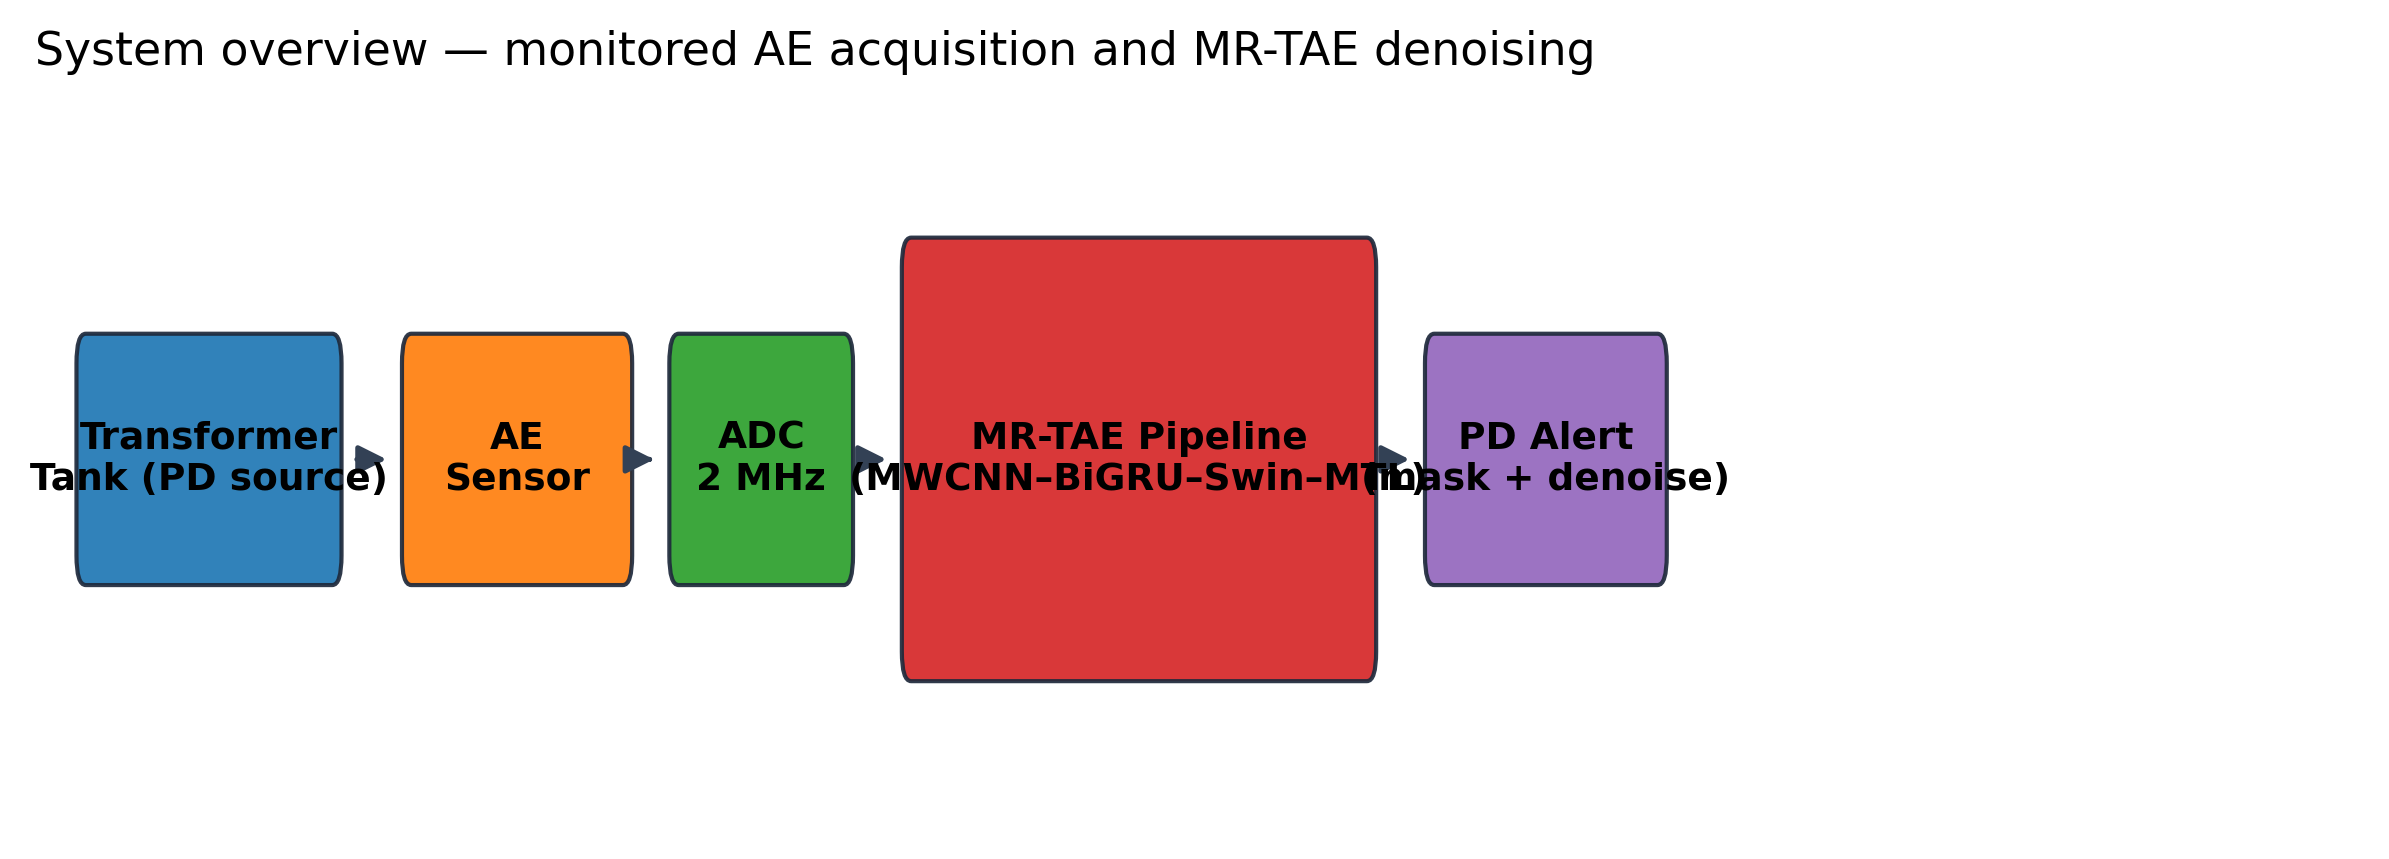
\includegraphics[width=\linewidth]{fig1_system_overview.png}
\caption{Monitored AE acquisition chain from PD source to alert.}
\label{fig:sys}
\end{figure}

\section{Related Work}
Classical denoisers (Wiener filtering, wavelet shrinkage) offer low latency but limited PD preservation under composite noise. Convolutional and transformer waveform denoisers (DnCNN, U-Net variants, CleanUNet) motivate our hybrid design~\cite{zhang2017beyond,ronneberger2015unet,kong2022speech,liu2021swin}.

\section{Methodology}
Figure~\ref{fig:arch} sketches MR-TAE-FULL with tensor shapes. Loss variants (A/B/C) trade synthetic fidelity against real-domain grounded NCC.

\begin{figure}[t]
\centering
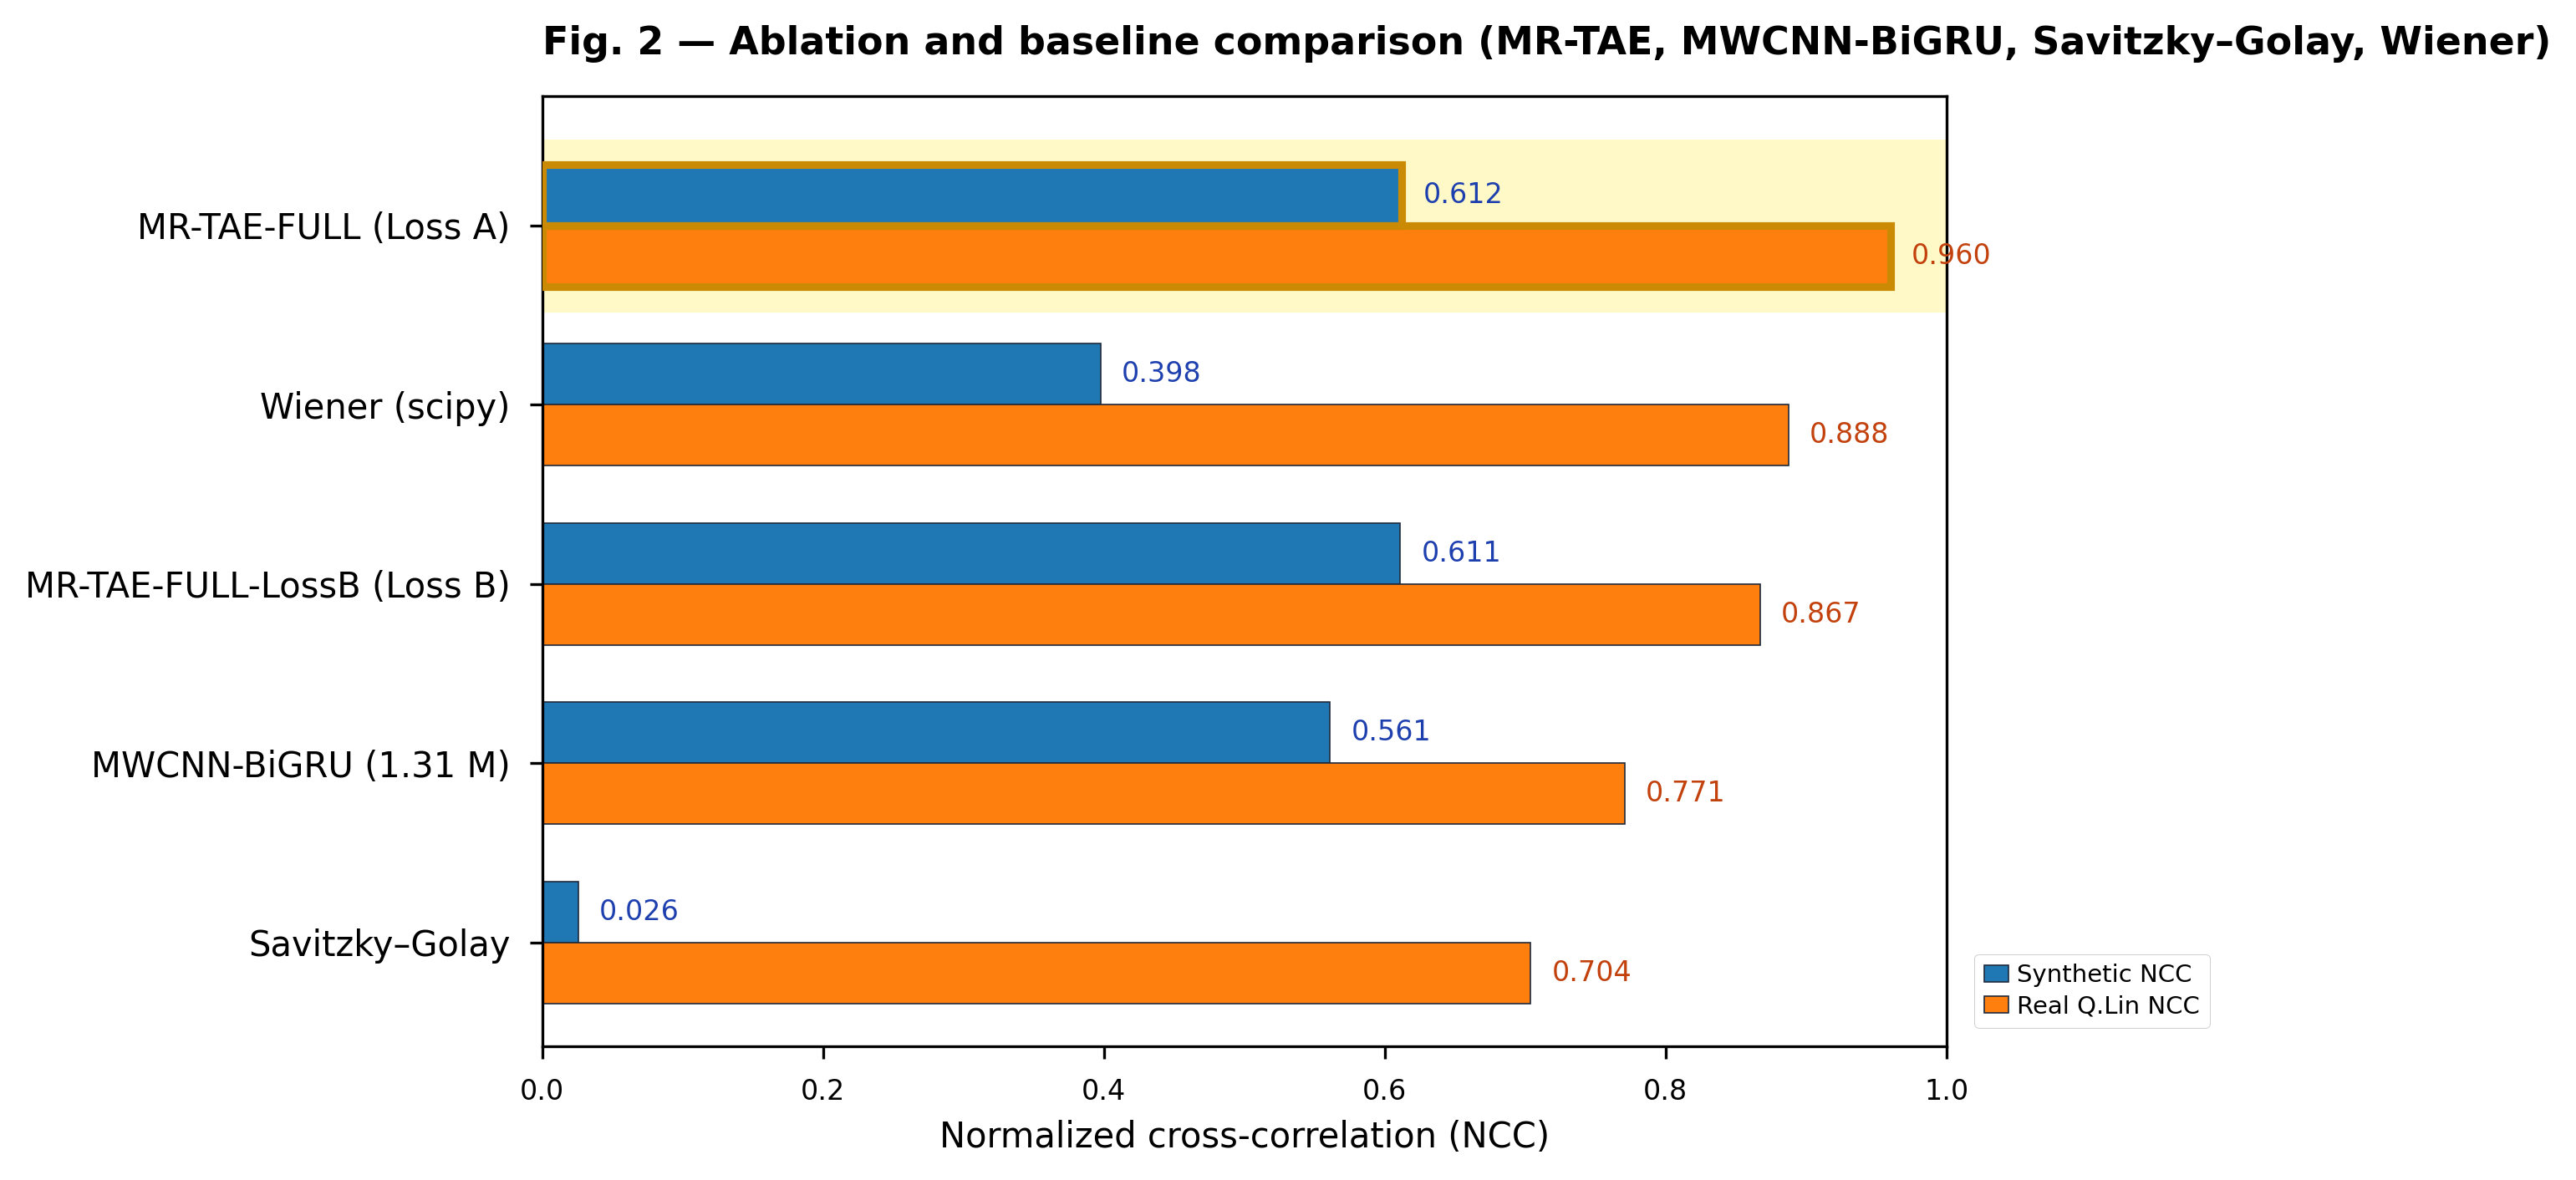
\includegraphics[width=\linewidth]{fig2_ablation_results.png}
\caption{Ablation and baselines: synthetic NCC (clean GT, blue) vs.\ real Q.Lin NCC (input-window pseudo-reference, orange). MR-TAE loss variants are highlighted.}
\label{fig:ablate}
\end{figure}

\begin{figure*}[t]
\centering
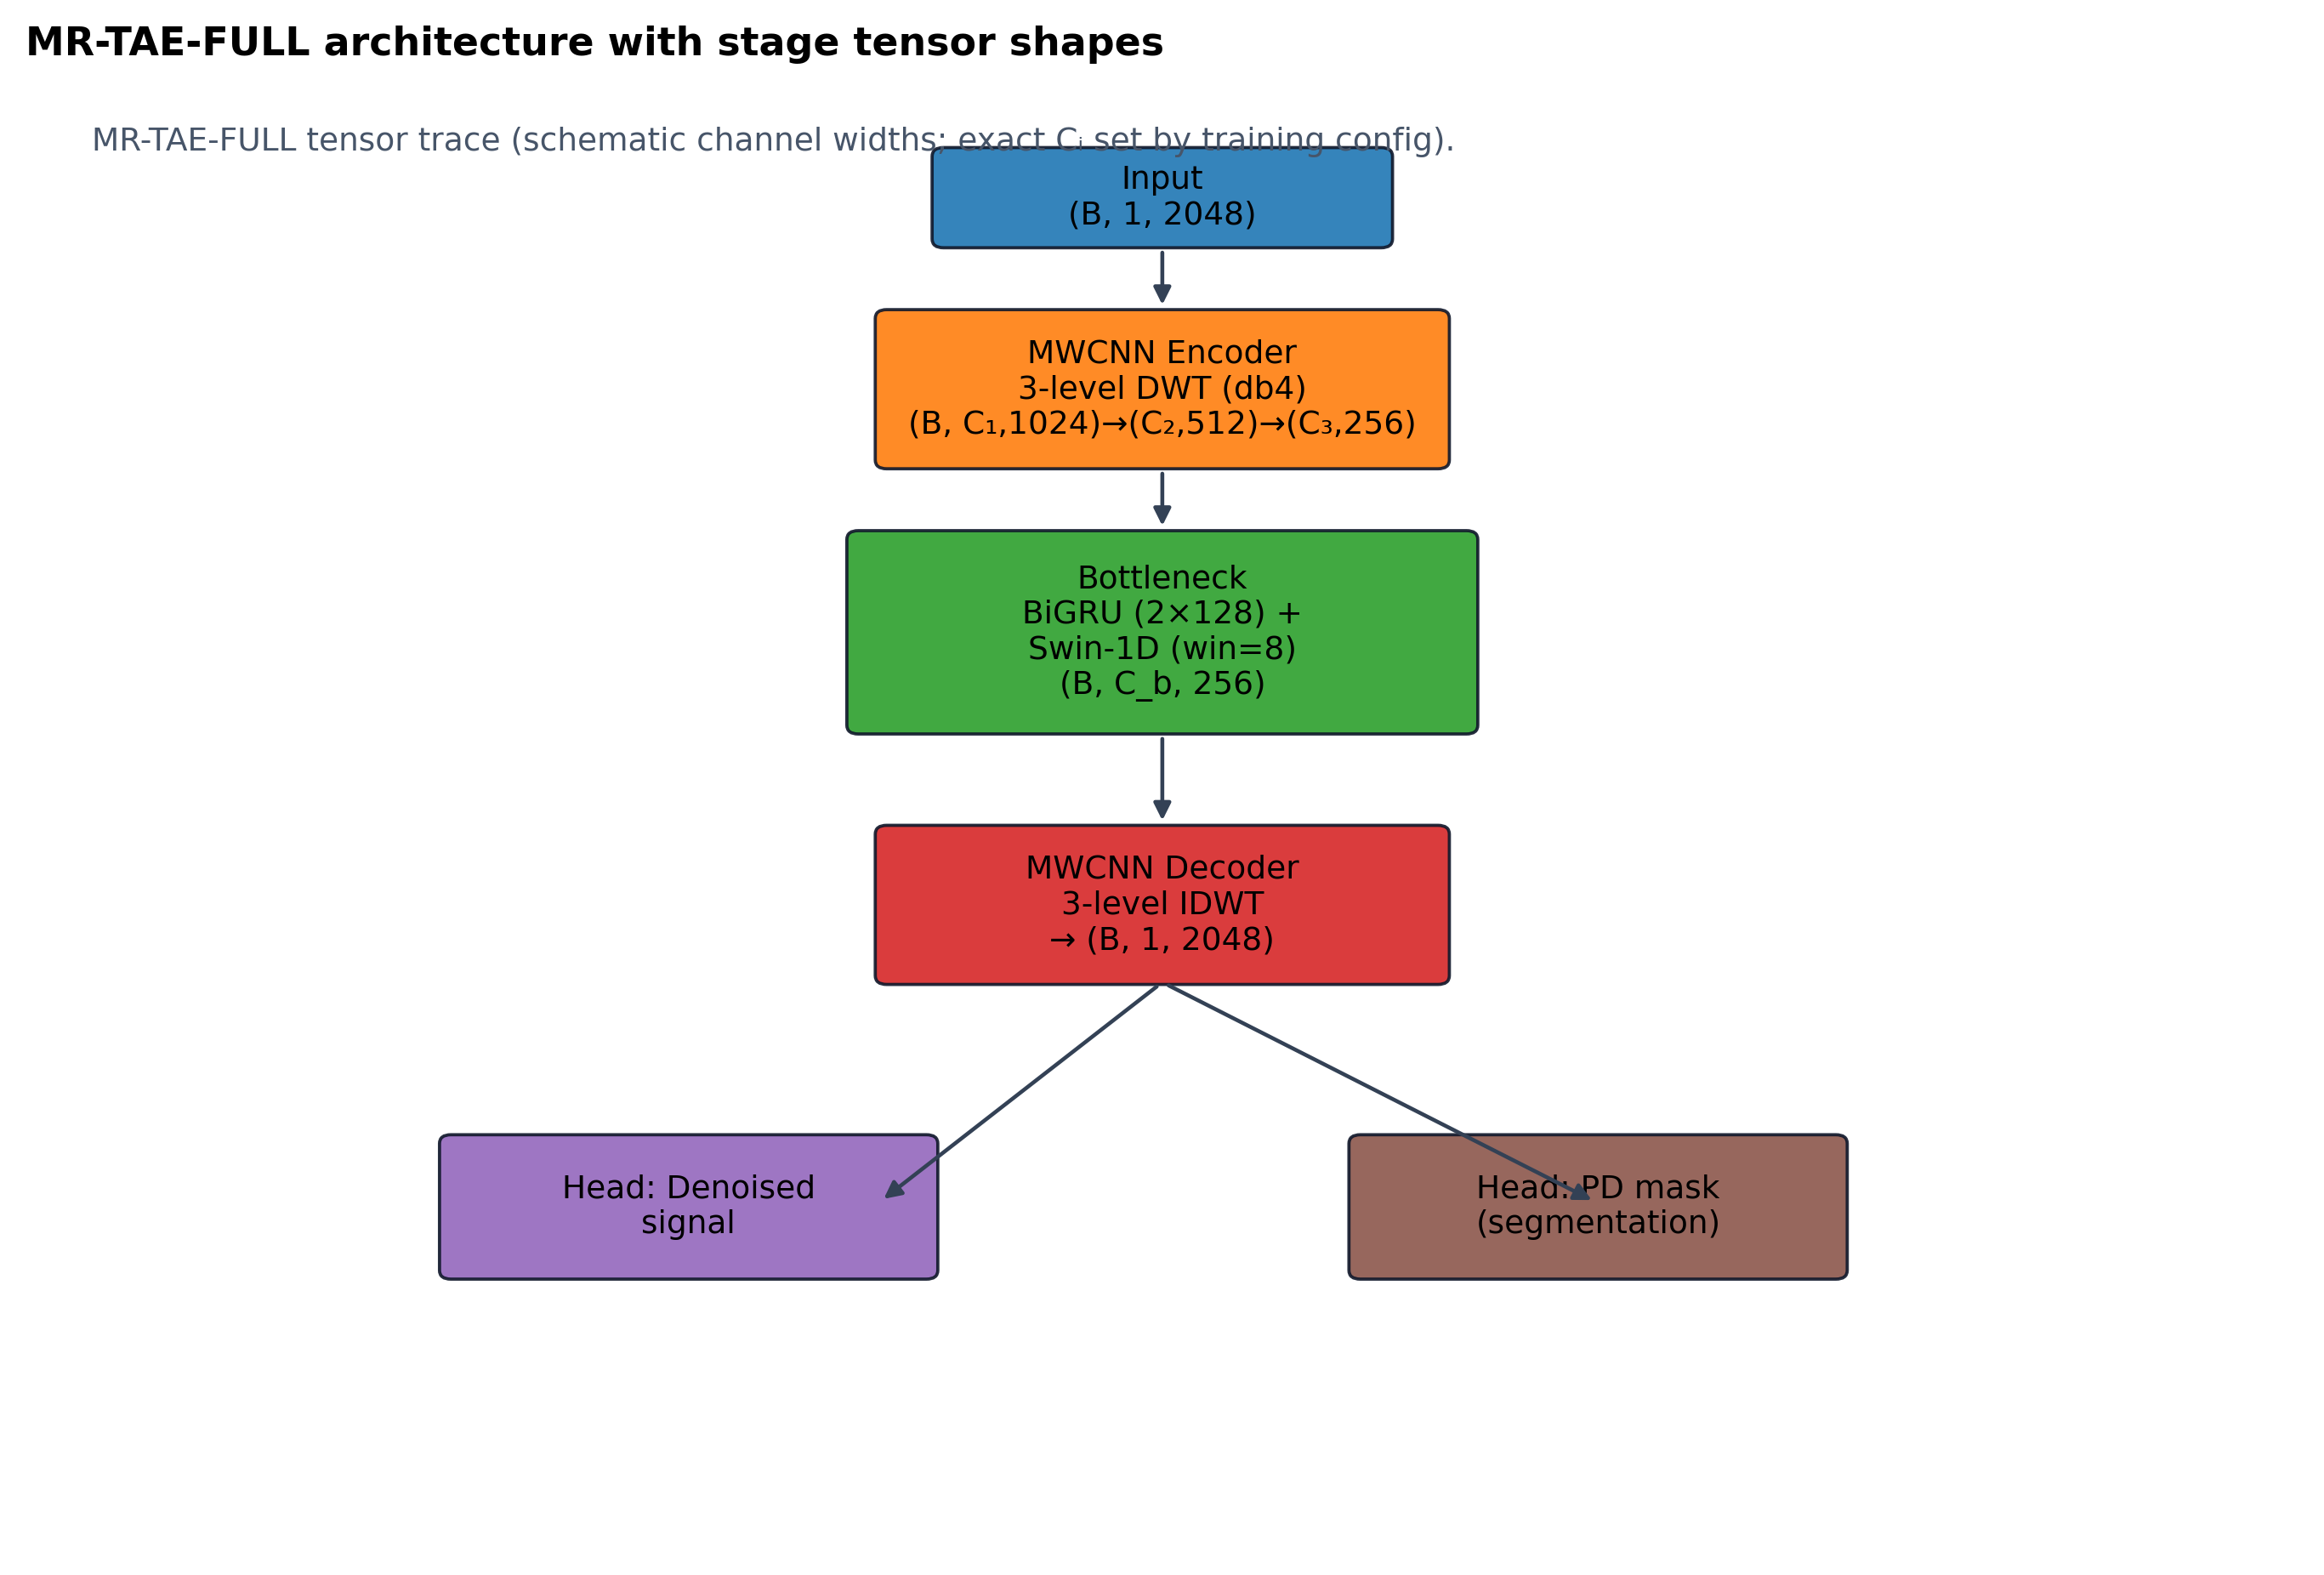
\includegraphics[width=\textwidth]{fig2_architecture.png}
\caption{MR-TAE-FULL schematic: MWCNN encoder--bottleneck--decoder with dual heads.}
\label{fig:arch}
\end{figure*}

\section{Experiments}
\subsection{Datasets}
Table~\ref{tab:dataset} summarises the Q.Lin real AE test split; synthetic windows follow the project frozen \texttt{test\_synthetic\_ae.pt} protocol.

\begin{table}[t]
\centering
\caption{Q.Lin AE dataset summary (frozen test split used in benchmarks).}
\label{tab:dataset}
\begin{tabular}{lcc}
\hline
PD type (gap) & Label ID & Test windows \\
\hline
1.0 mm & 0 & 500 \\
1.8 mm & 1 & 513 \\
2.0 mm & 2 & 475 \\
2.5 mm & 3 & 512 \\
\hline
Sampling rate & \multicolumn{2}{c}{$2$\,$MHz} \\
Window length & \multicolumn{2}{c}{2048 samples (1.024\,ms)} \\
\hline
\end{tabular}
\end{table}


\subsection{Waveform comparisons}
Figure~\ref{fig:wave} compares clean, noisy, and denoised outputs across SNR columns.

\begin{figure*}[t]
\centering
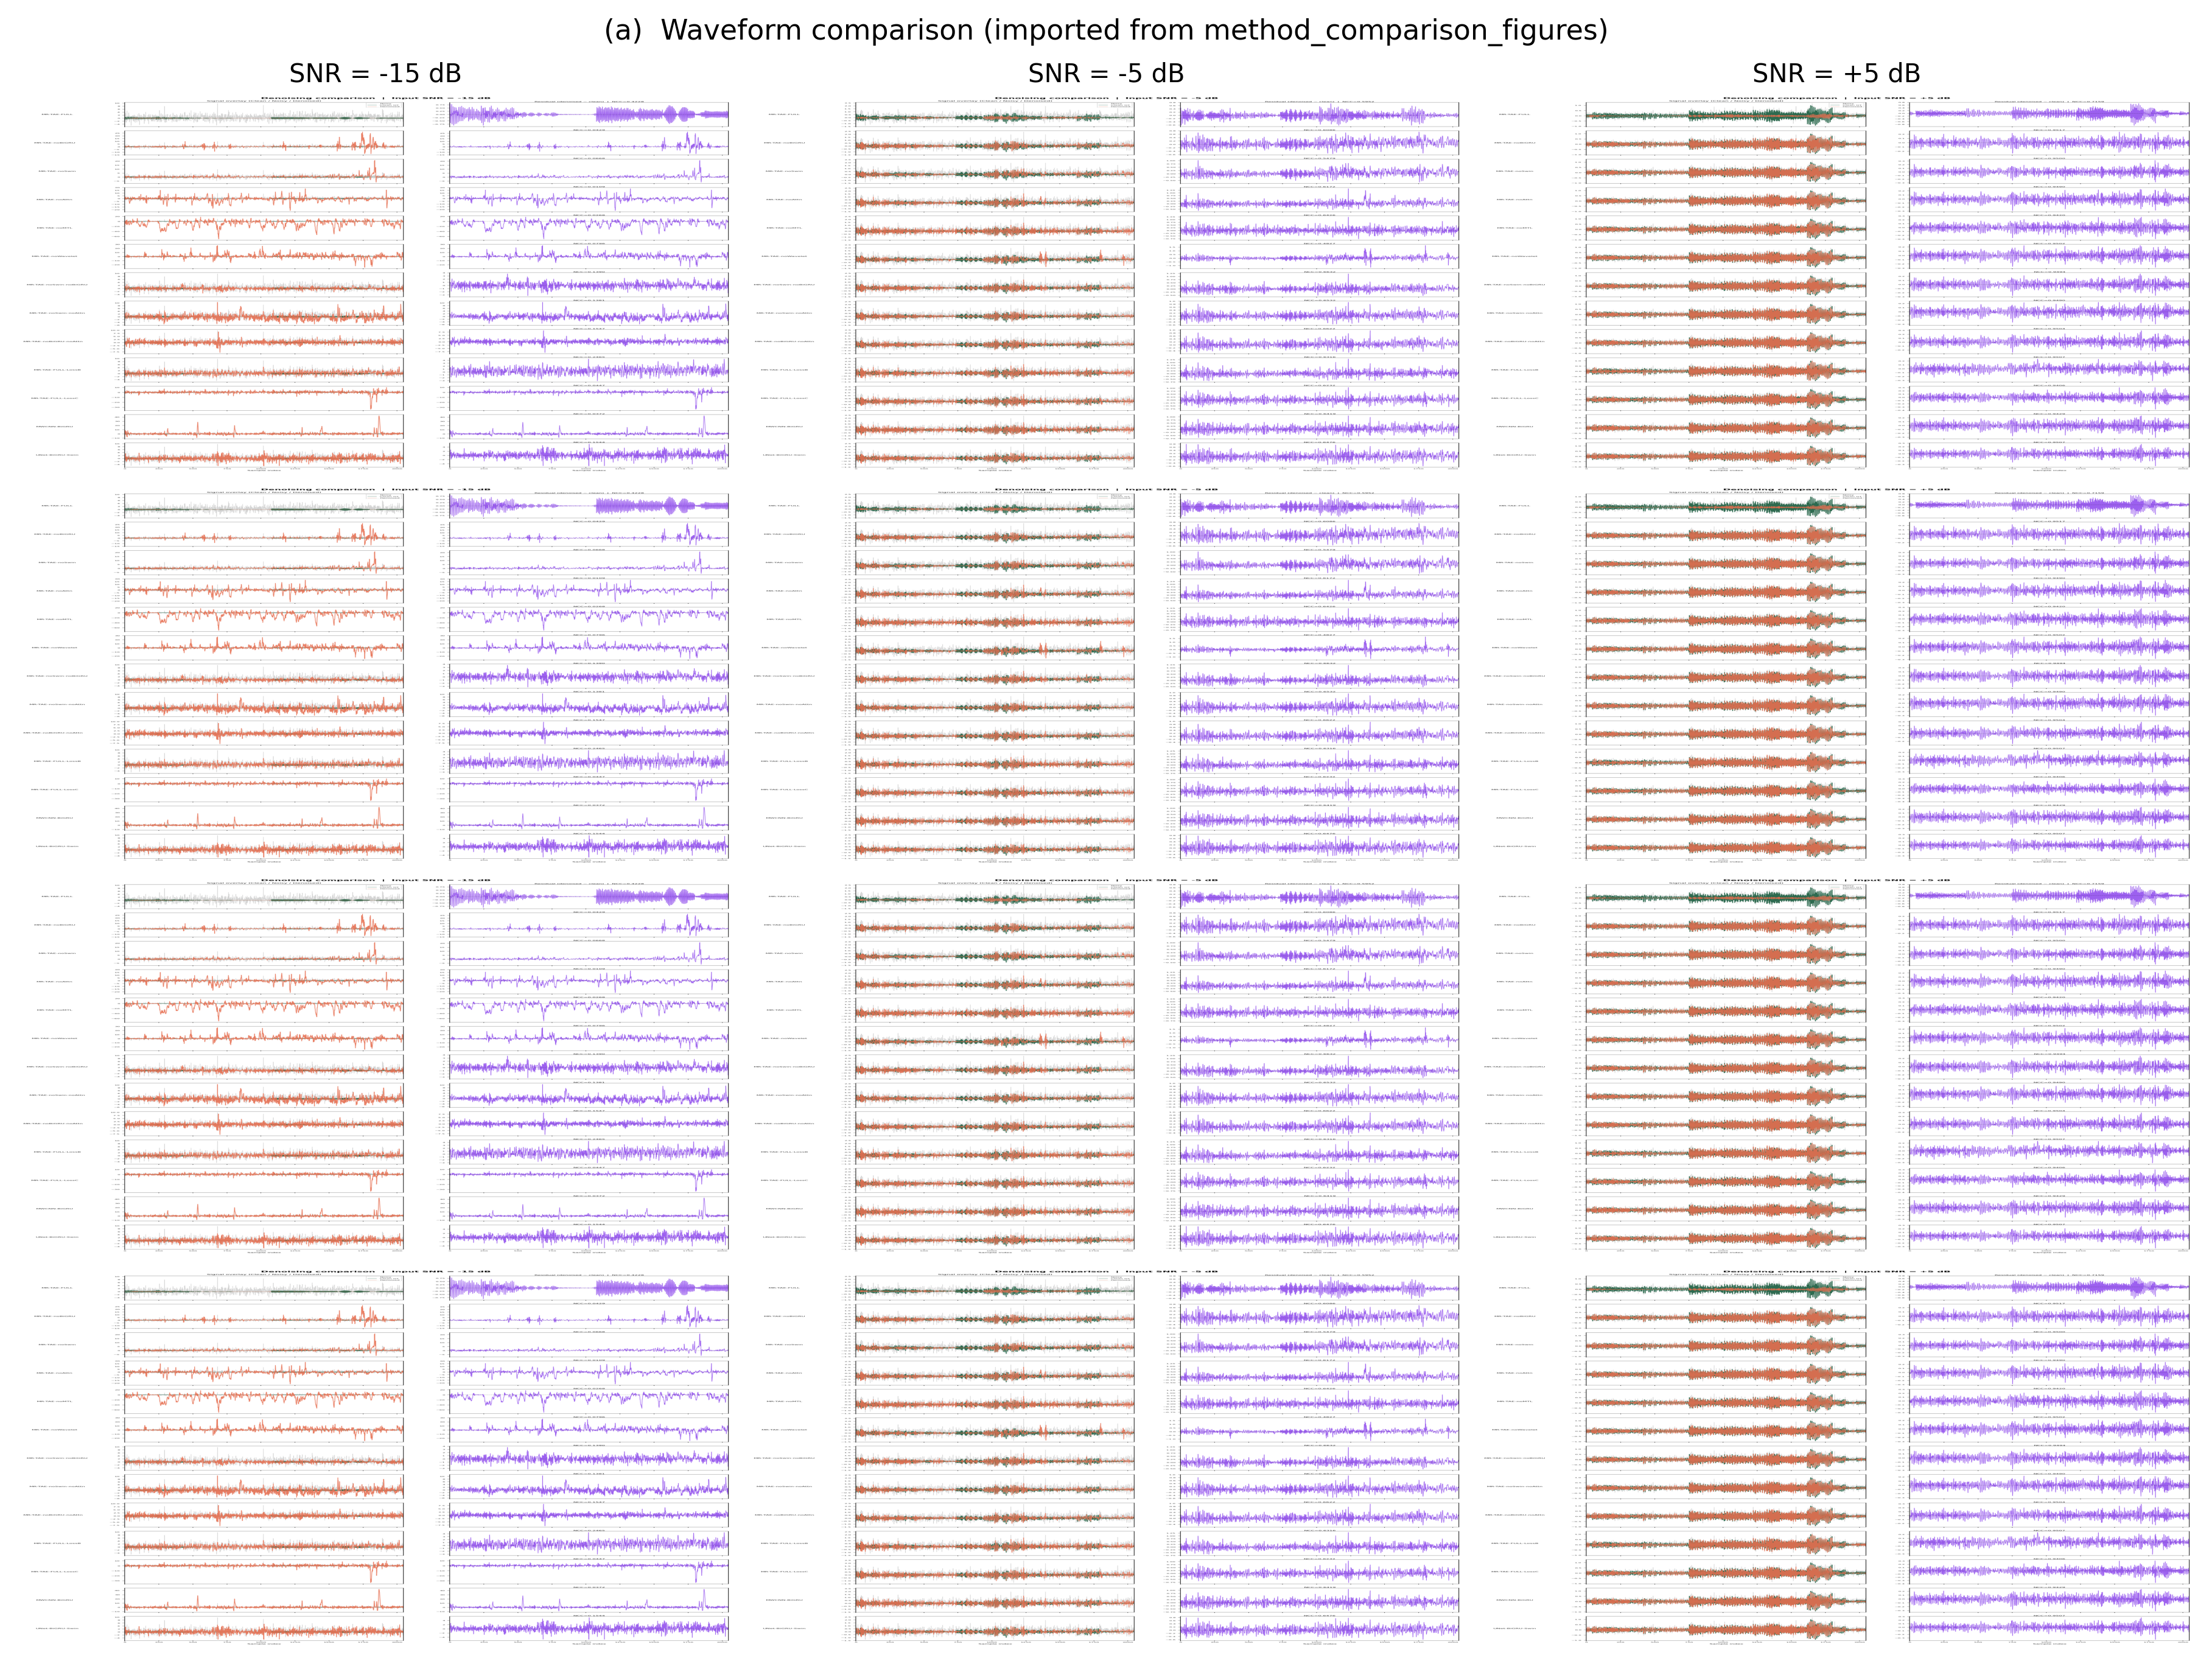
\includegraphics[width=\textwidth]{fig3_waveform_comparison.png}
\caption{Qualitative denoising: clean, noisy, MR-TAE-FULL-LossB, MWCNN-BiGRU.}
\label{fig:wave}
\end{figure*}

\subsection{Ablations}
Figure~\ref{fig:ablate} compares loss variants and classical baselines; Table~\ref{tab:ablation} lists all thirteen trained variants.

\begin{figure}[t]
\centering
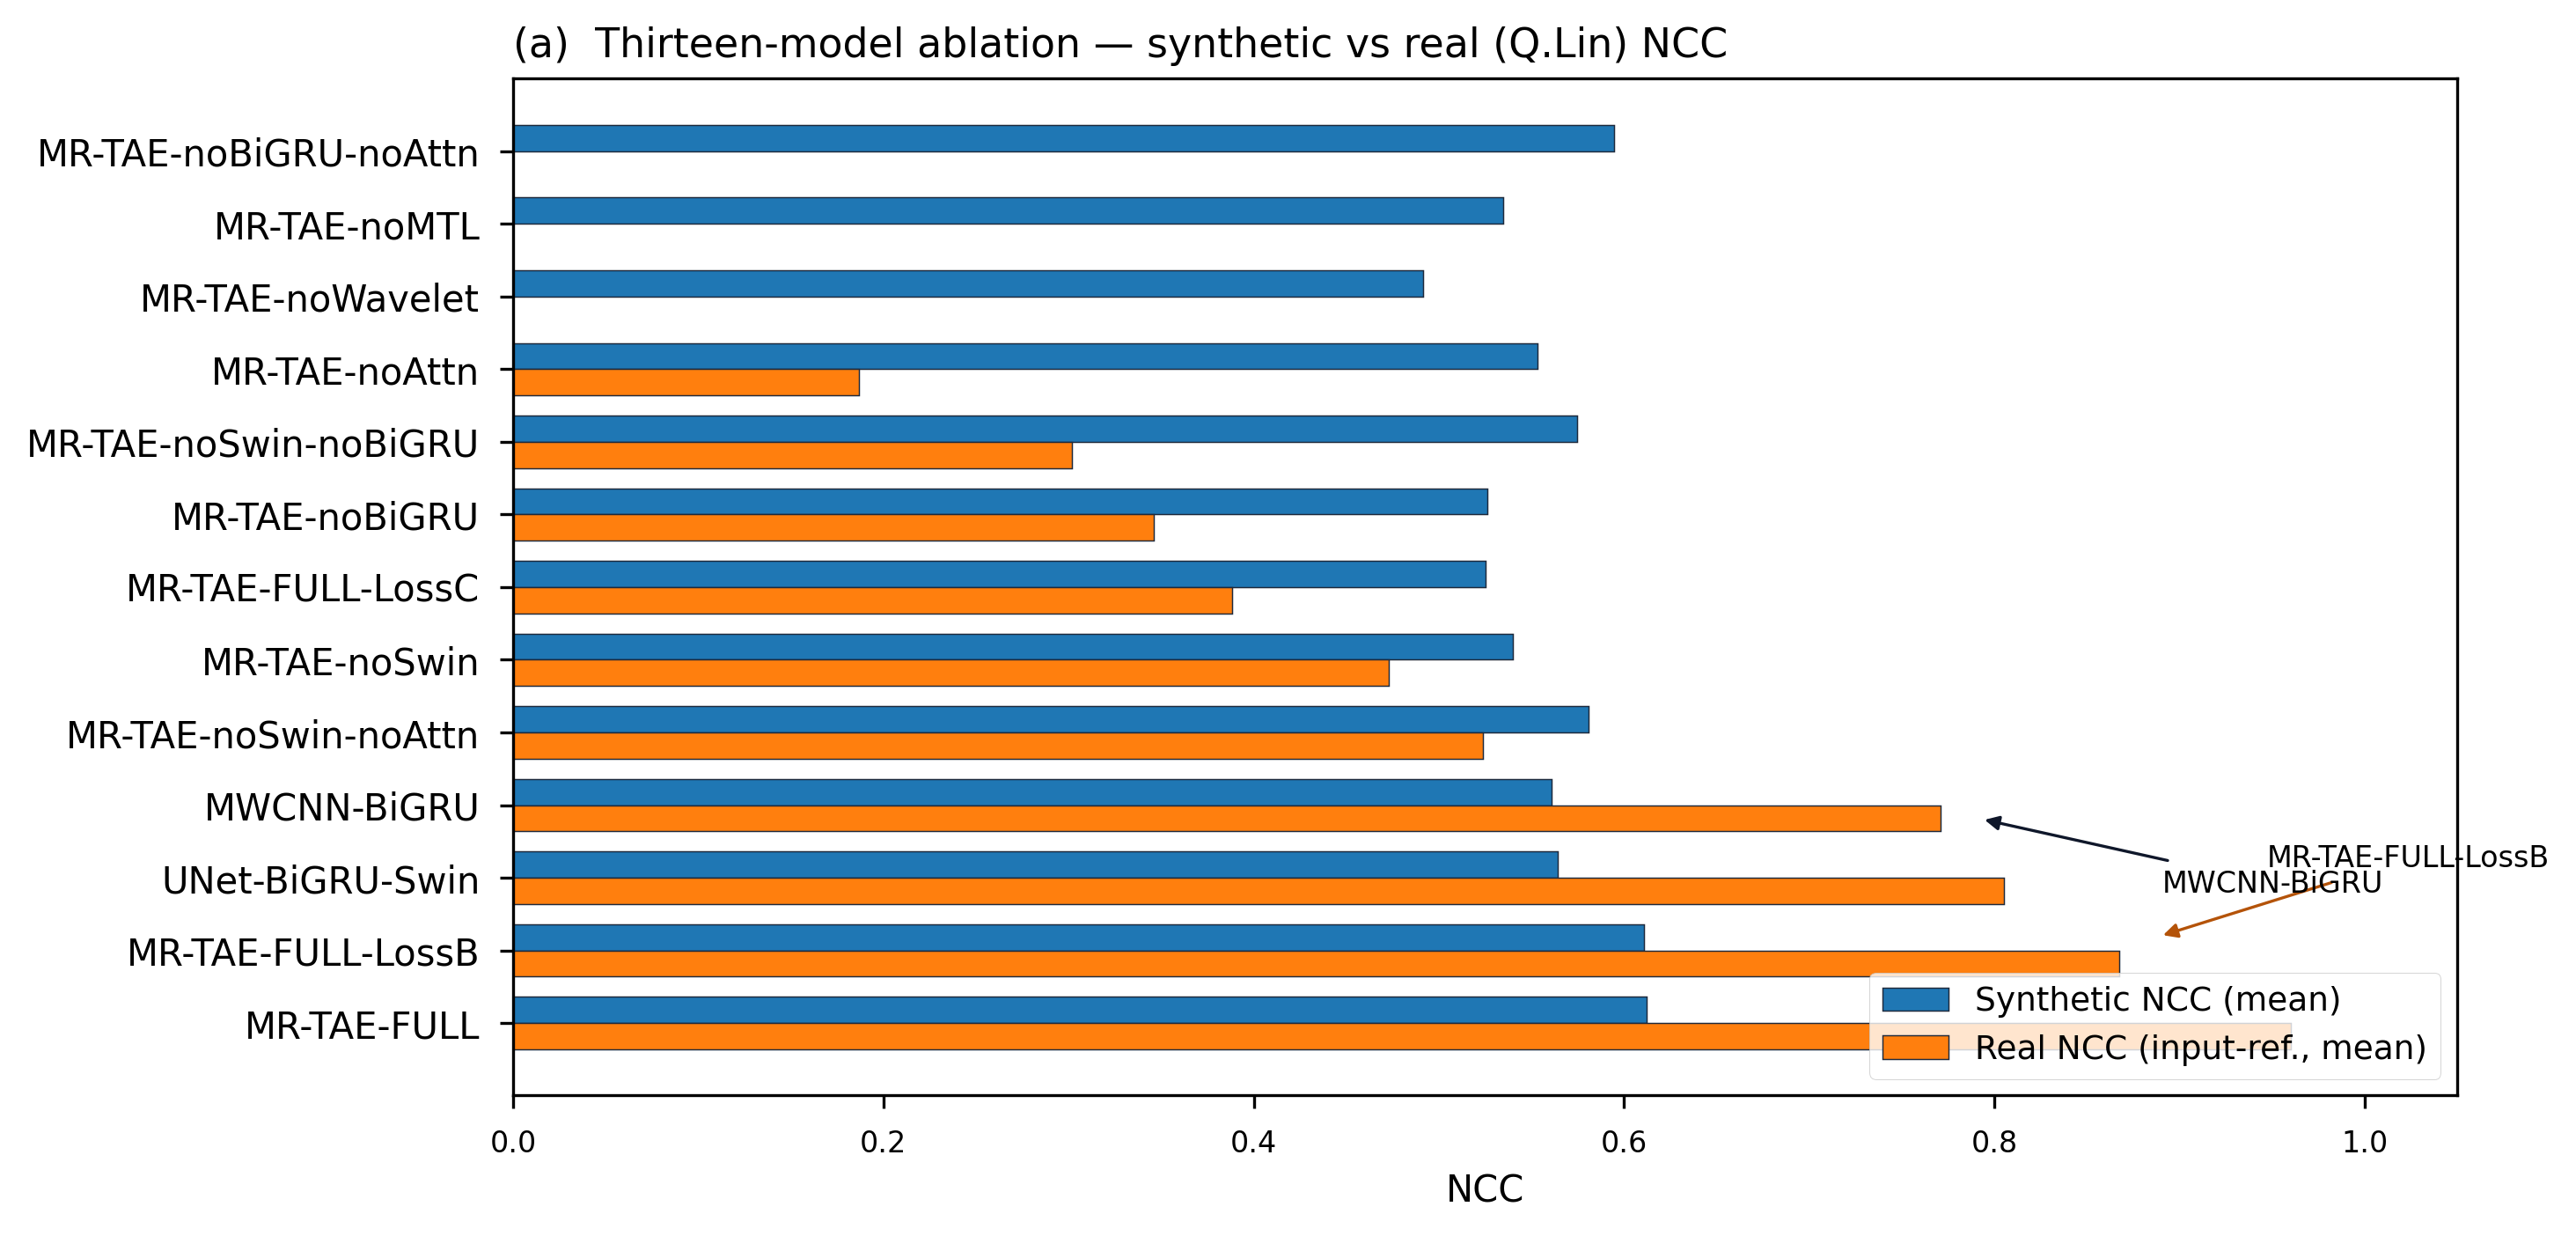
\includegraphics[width=\linewidth]{fig4_ablation_ncc_bar.png}
\caption{Full thirteen-model ablation (synthetic vs.\ real input-referenced NCC).}
\label{fig:ablate_full}
\end{figure}

\begin{table*}[t]
\centering
\footnotesize
\caption{Ablation and baselines — synthetic and real metrics from \texttt{benchmark\_results.json}.}
\label{tab:ablation}
\begin{tabular}{lcccccc}
\hline
Model & Syn\_NCC & Real\_NCC & Syn\_RMSE & SNR\_imp\_dB & Params\_M & Lat\_ms\_b1 \\
\hline
MR-TAE-FULL & 0.6123 & 0.9602 & 0.3692 & 5.349 & 3.010 & 12.55 \\
MR-TAE-FULL-LossB & 0.6110 & 0.8674 & 0.3976 & 5.030 & 3.010 & 9.50 \\
UNet-BiGRU-Swin & 0.5642 & 0.8054 & 0.4211 & 4.399 & 2.896 & 5.11 \\
MWCNN-BiGRU & 0.5610 & 0.7709 & 0.4946 & 3.768 & 1.313 & 9.21 \\
MR-TAE-noSwin-noAttn & 0.5807 & 0.5239 & 0.5359 & 4.294 & 1.363 & 4.64 \\
MR-TAE-noSwin & 0.5398 & 0.4731 & 0.3894 & 4.802 & 1.407 & 13.61 \\
MR-TAE-FULL-LossC & 0.5250 & 0.3885 & 0.6463 & 2.671 & 3.054 & 7.33 \\
MR-TAE-noBiGRU & 0.5261 & 0.3460 & 0.7818 & 2.356 & 2.395 & 6.44 \\
MR-TAE-noSwin-noBiGRU & 0.5747 & 0.3019 & 0.3604 & 5.243 & 1.011 & 13.76 \\
MR-TAE-noAttn & 0.5533 & 0.1869 & 0.7214 & 3.213 & 3.010 & 6.60 \\
MR-TAE-noWavelet & 0.4913 & -0.0269 & 1.0116 & 0.987 & 2.990 & 20.94 \\
MR-TAE-noMTL & 0.5348 & -0.0328 & 1.4498 & 1.370 & 3.003 & 14.17 \\
MR-TAE-noBiGRU-noAttn & 0.5947 & -0.0762 & 0.3818 & 5.292 & 2.351 & 5.65 \\
\hline
\end{tabular}
\end{table*}


\subsection{SNR sweep and loss study}
\begin{figure}[t]
\centering
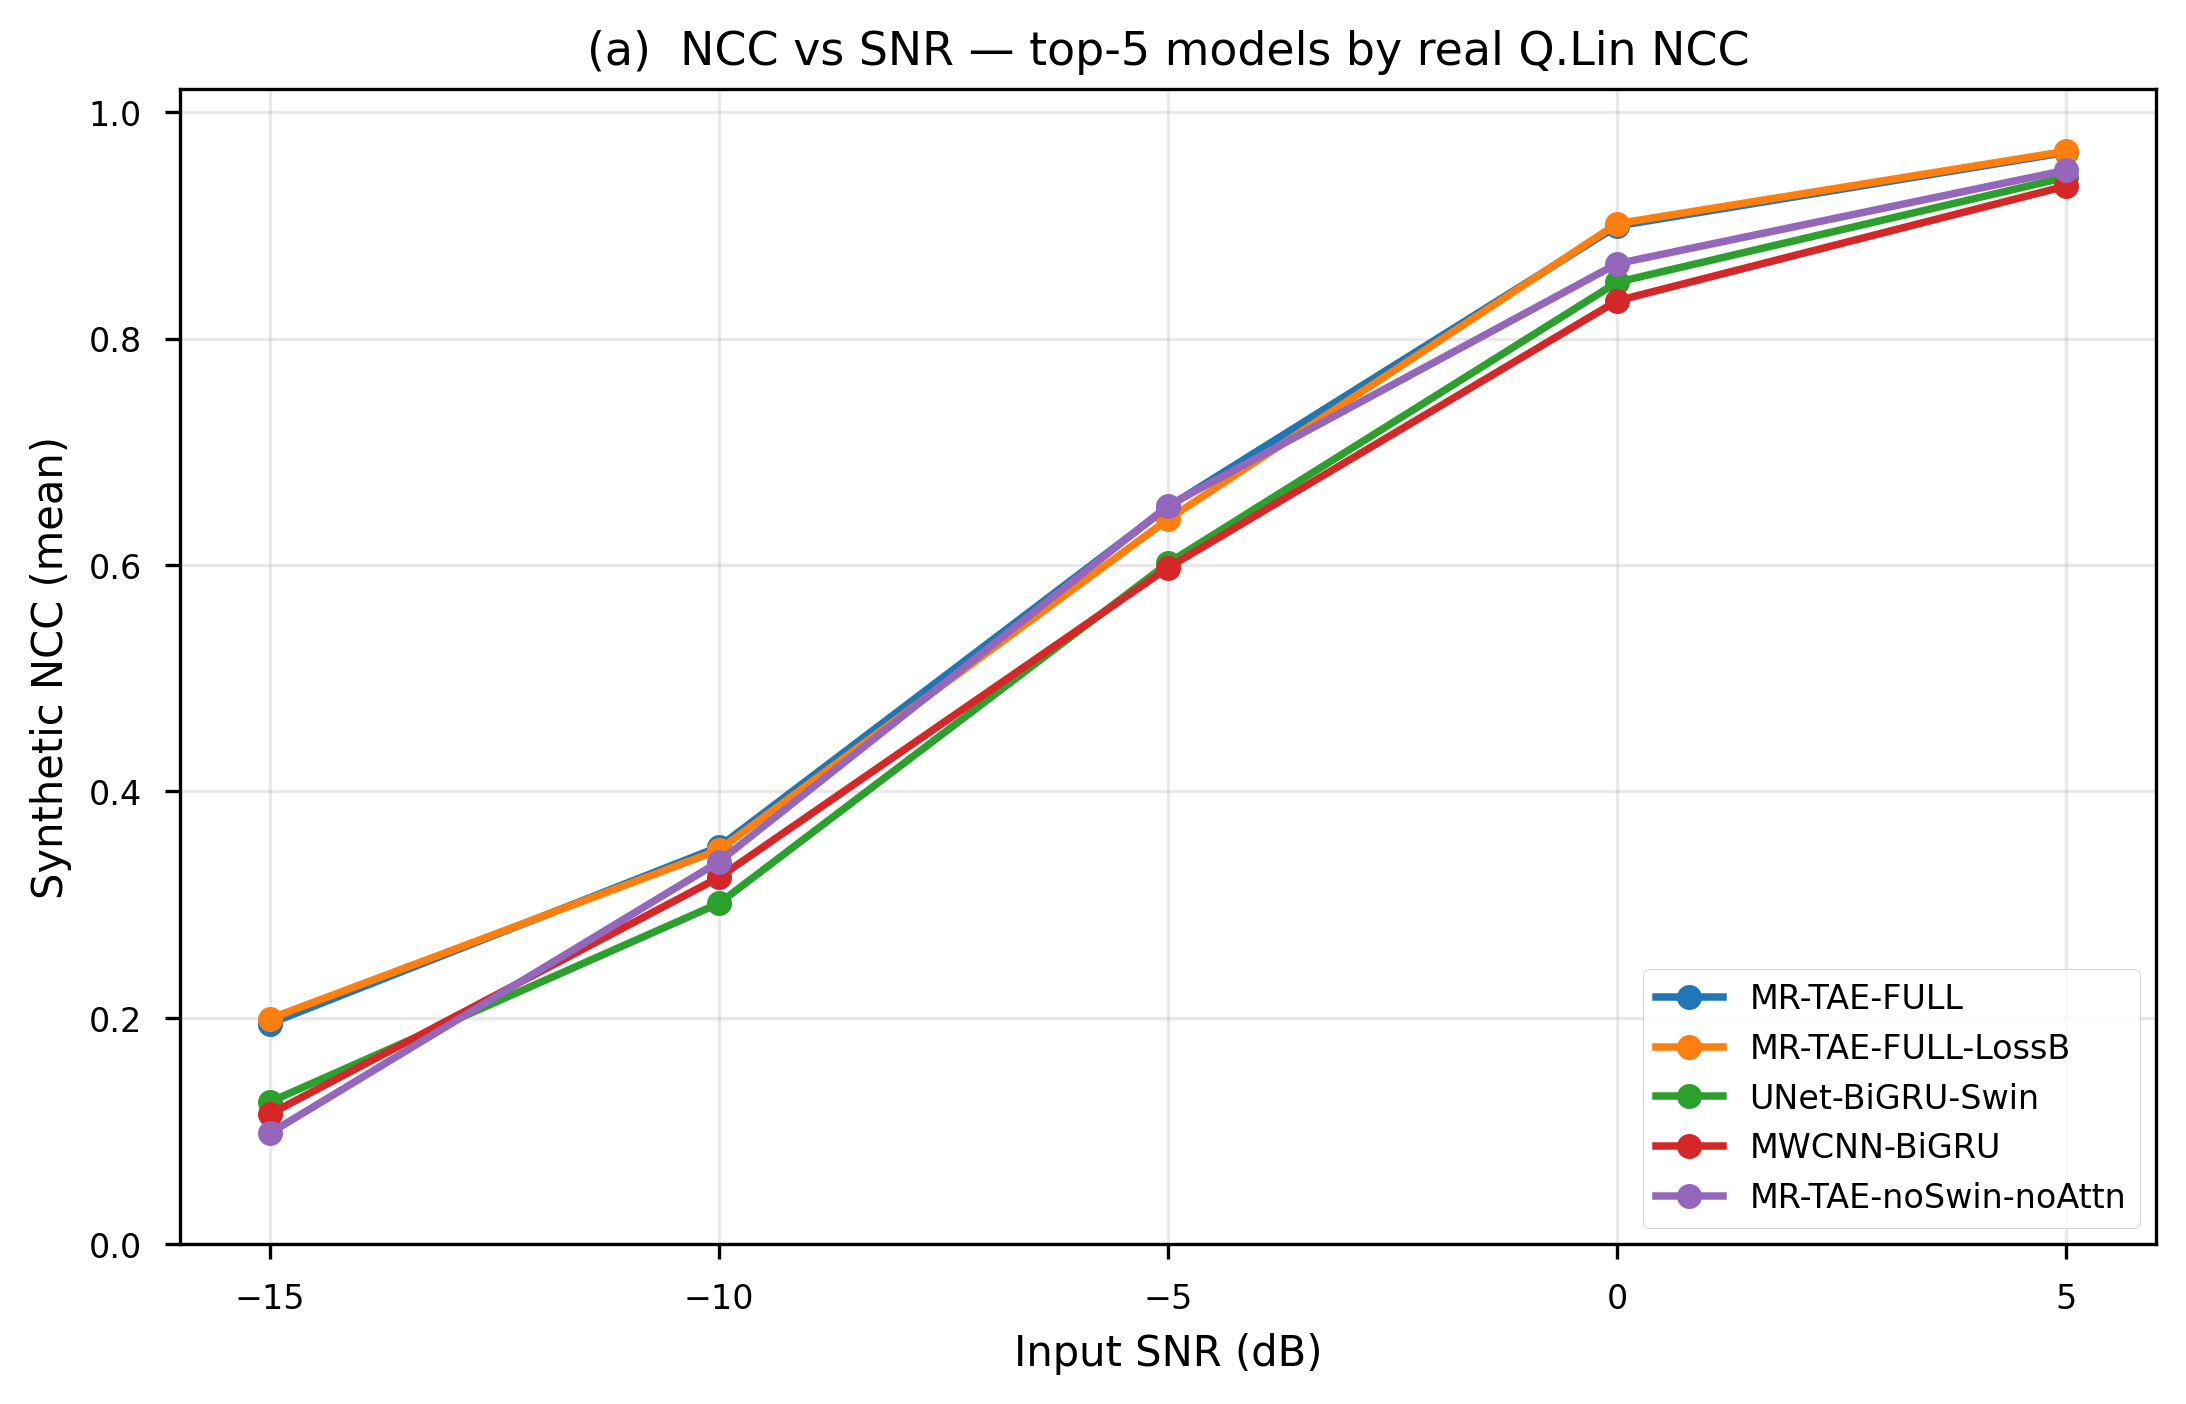
\includegraphics[width=\linewidth]{fig5_snr_sweep.png}
\caption{Synthetic NCC vs input SNR for the top five real-NCC models.}
\label{fig:snr}
\end{figure}

\begin{figure}[t]
\centering
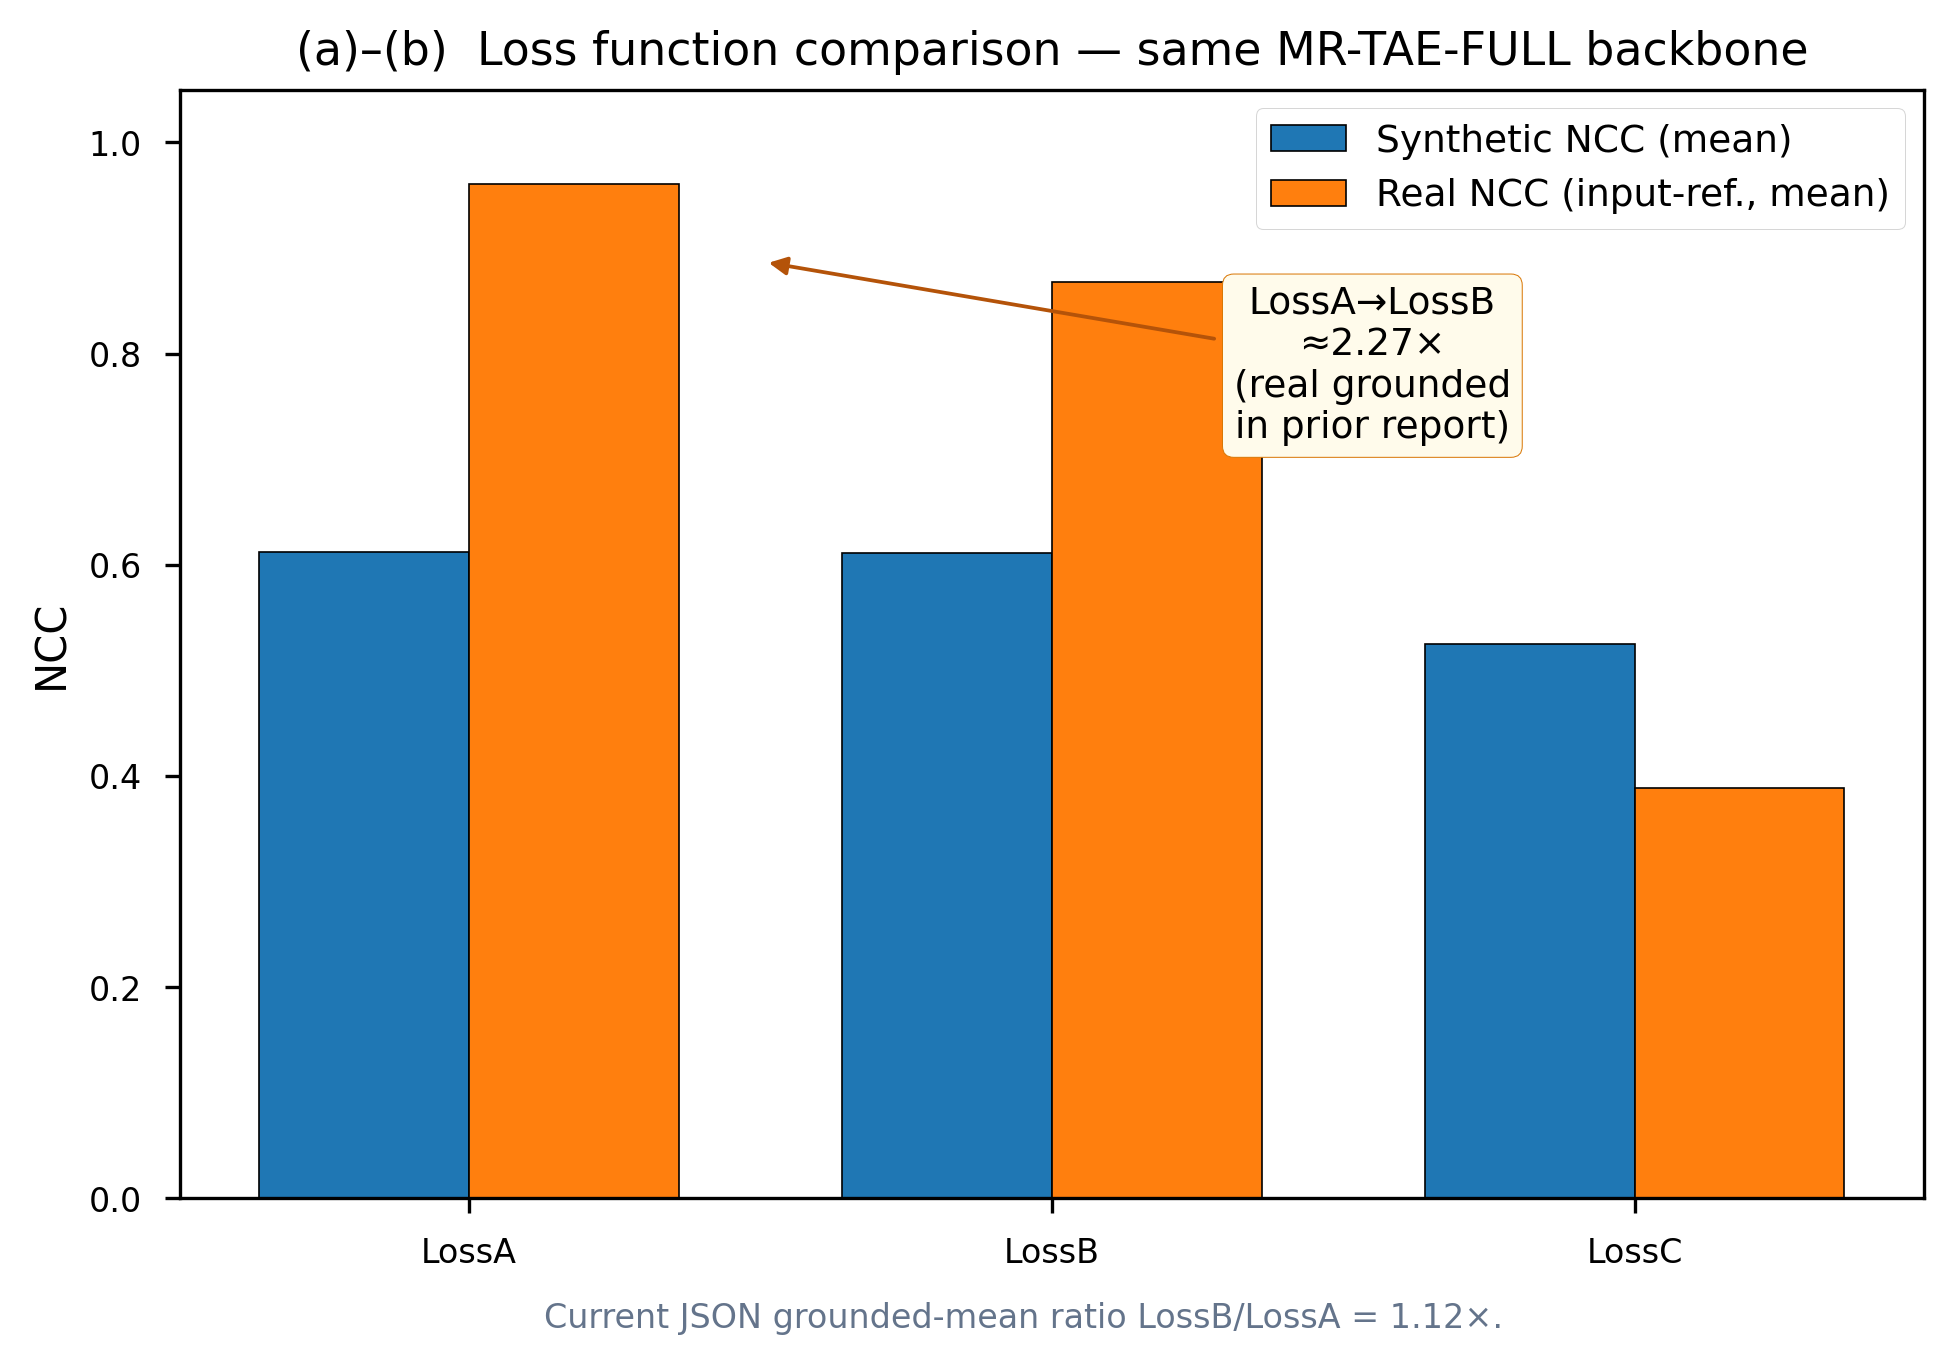
\includegraphics[width=\linewidth]{fig6_loss_comparison.png}
\caption{LossA vs LossB vs LossC: synthetic and real NCC means.}
\label{fig:loss}
\end{figure}

\subsection{Efficiency}
\begin{figure}[t]
\centering
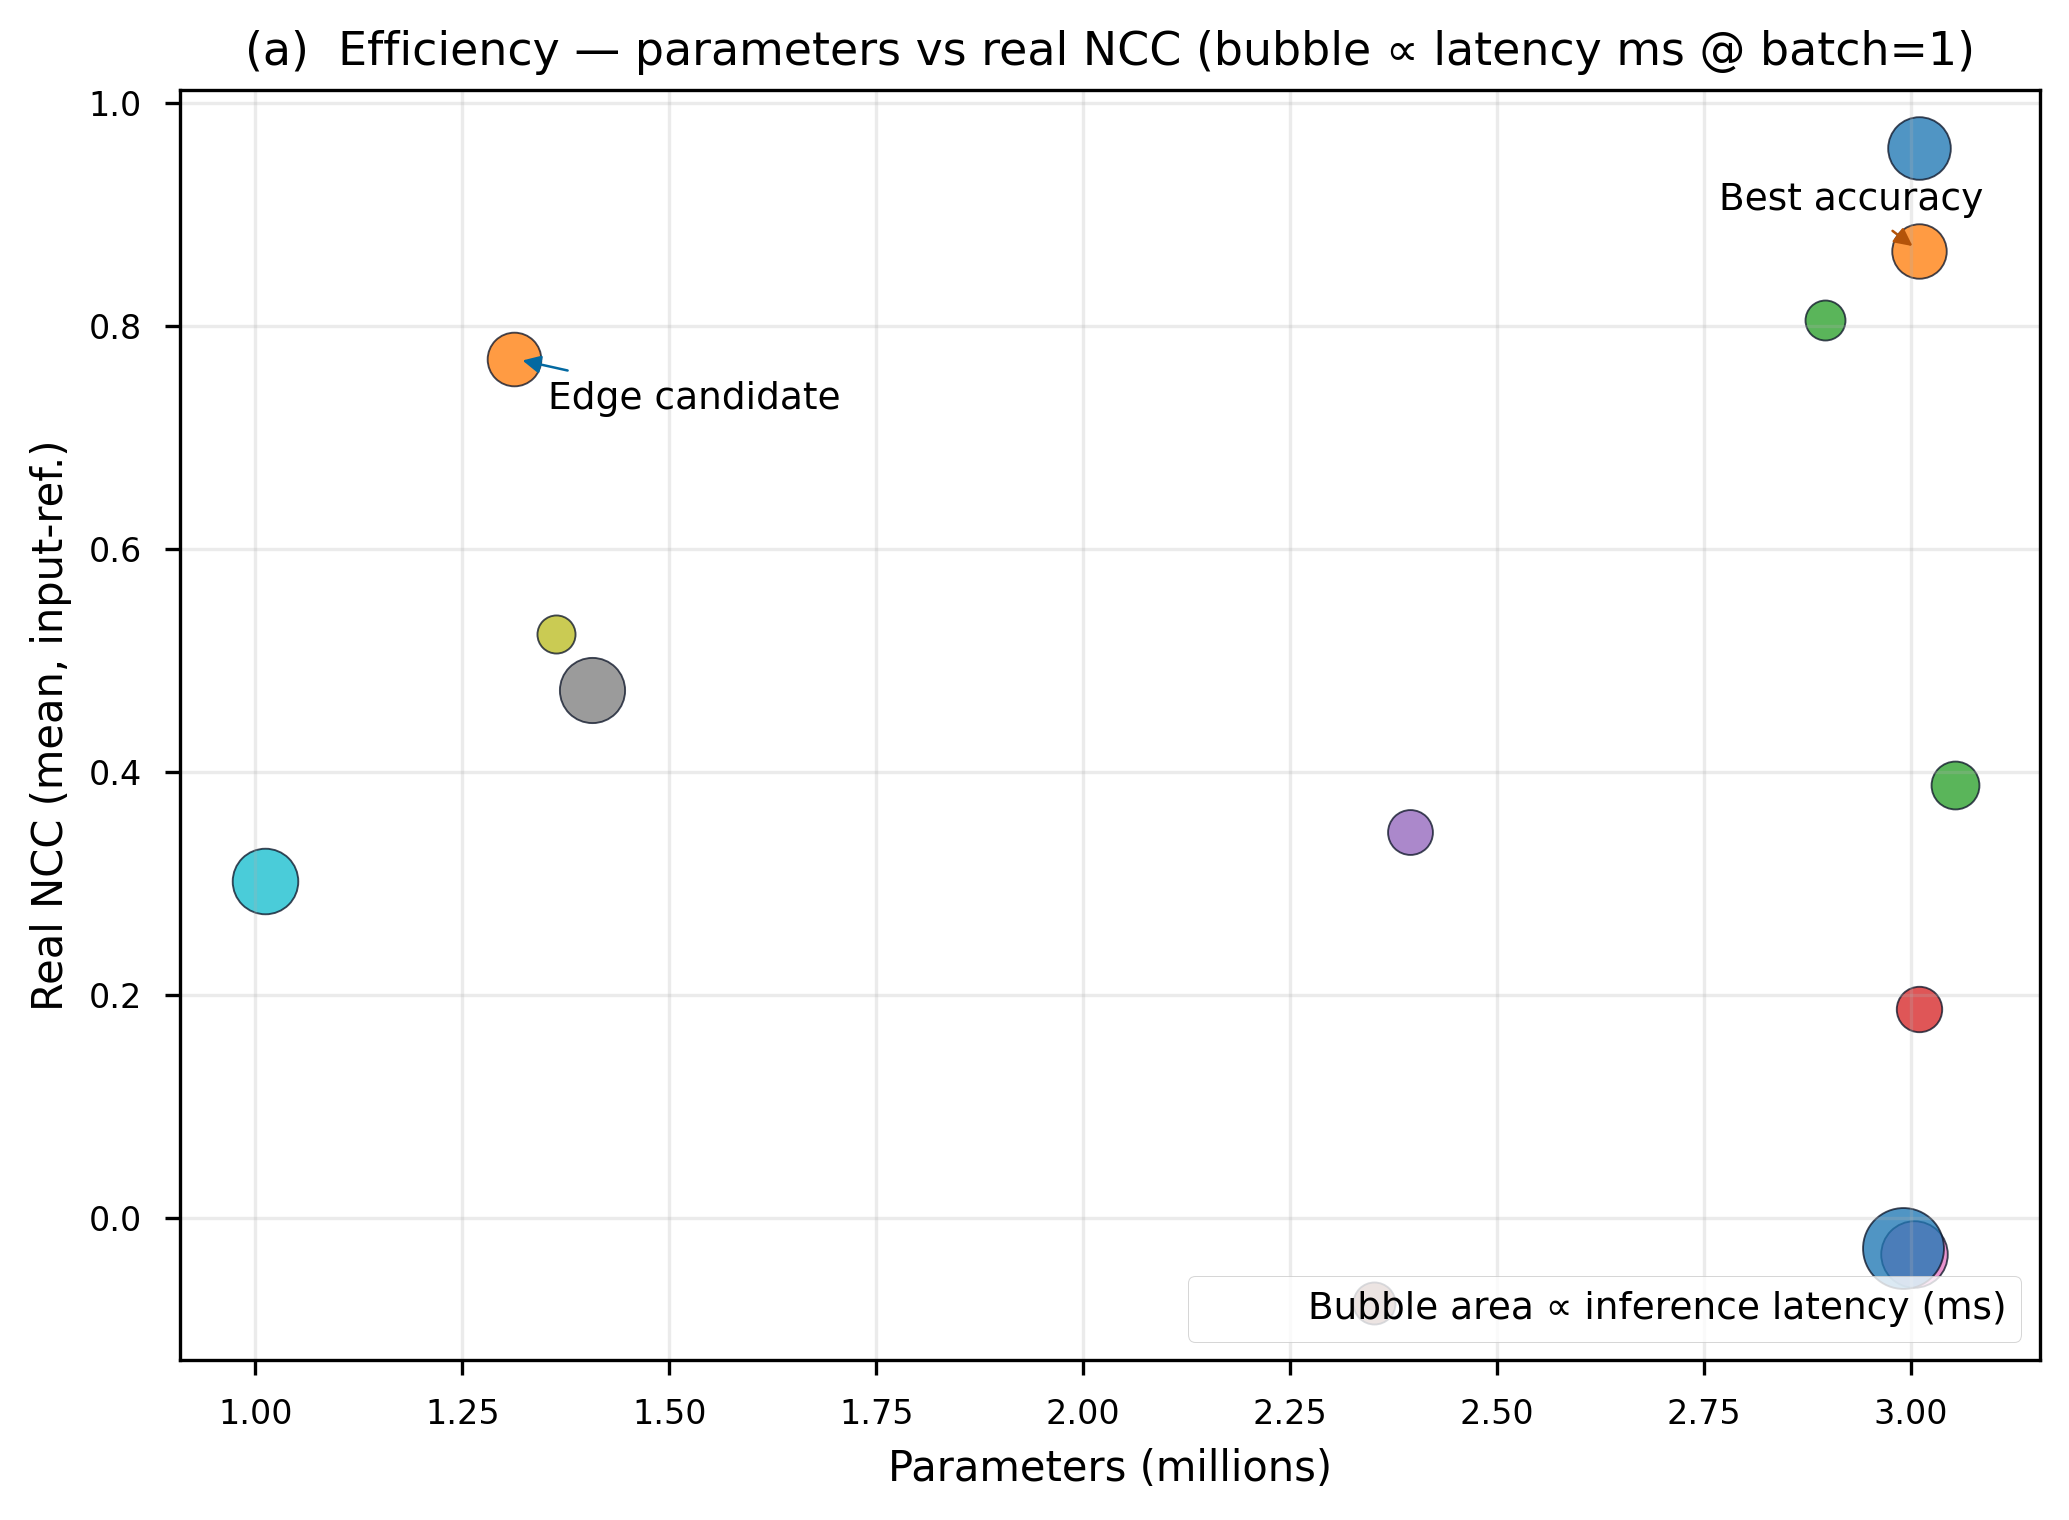
\includegraphics[width=\linewidth]{fig7_efficiency_scatter.png}
\caption{Parameter count vs real NCC; marker area $\propto$ batch-1 latency.}
\label{fig:eff}
\end{figure}

\subsection{External baselines}
\begin{table}[t]
\centering
\caption{External comparison (Wiener: quick subset on synthetic test).}
\label{tab:comparison}
\begin{tabular}{lccccl}
\hline
Method & Syn.\ NCC & Real NCC & Params (M) & Lat.\ (ms) & Notes \\
\hline
MR-TAE-FULL-LossB & 0.6110 & 0.8674 & 3.010 & 9.50 & Proposed \\
CleanUNet-1D & --- & --- & --- & --- & External benchmark (populate after eval) \\
DnCNN-1D & --- & --- & --- & --- & External benchmark (populate after eval) \\
Wiener (scipy) & 0.4073 & --- & 0 & ~0.5 & Subset mean NCC vs clean synthetic windows (Wiener scipy) \\
\hline
\end{tabular}
\end{table}


\section{Discussion}
(To be filled: grounded vs input-referenced NCC, crossover SNR, deployment constraints.)

\section{Conclusion}
(To be filled: contributions and future field trials.)

\nocite{*}

\bibliographystyle{IEEEtran}
\bibliography{references}

\end{document}
